\documentclass[letterpaper,10pt]{article}

\usepackage{titling}
\usepackage{listings}
\usepackage{url}
\usepackage{setspace}
\usepackage{subfig}
\usepackage{sectsty}
\usepackage{pdfpages}
\usepackage{colortbl}
\usepackage{multirow}
\usepackage{multicol}
\usepackage{relsize}
\usepackage{amsmath}
\usepackage{wasysym}
\usepackage{fancyvrb}
\usepackage{amssymb}
\usepackage{ifsym}
\usepackage{amsmath,amssymb,amsthm,graphicx,xspace}
\usepackage[titlenotnumbered,noend,noline]{algorithm2e}
\usepackage[compact]{titlesec}
\usepackage{XCharter}
\usepackage[T1]{fontenc}
\usepackage{tikz}
\usetikzlibrary{arrows,automata,shapes,trees,matrix,chains,scopes,positioning,calc}
\tikzstyle{block} = [rectangle, draw, fill=blue!20, 
    text width=2.5em, text centered, rounded corners, minimum height=2em]
\tikzstyle{bw} = [rectangle, draw, fill=blue!20, 
    text width=4em, text centered, rounded corners, minimum height=2em]

\definecolor{namerow}{cmyk}{.40,.40,.40,.40}
\definecolor{namecol}{cmyk}{.40,.40,.40,.40}

\let\LaTeXtitle\title
\renewcommand{\title}[1]{\LaTeXtitle{\textsf{#1}}}


\newcommand{\handout}[5]{
  \noindent
  \begin{center}
  \framebox{
    \vbox{
      \hbox to 5.78in { {\bf ECE356: Database Systems } \hfill #2 }
      \vspace{4mm}
      \hbox to 5.78in { {\Large \hfill #4  \hfill} }
      \vspace{2mm}
      \hbox to 5.78in { {\em #3 \hfill} }
    }
  }
  \end{center}
  \vspace*{4mm}
}

\newcommand{\lecture}[3]{\handout{#1}{#2}{#3}{Lecture #1}}
\newcommand{\tuple}[1]{\ensuremath{\left\langle #1 \right\rangle}\xspace}

\addtolength{\oddsidemargin}{-1.000in}
\addtolength{\evensidemargin}{-0.500in}
\addtolength{\textwidth}{2.0in}
\addtolength{\topmargin}{-1.000in}
\addtolength{\textheight}{1.75in}
\addtolength{\parskip}{\baselineskip}
\setlength{\parindent}{0in}
\renewcommand{\baselinestretch}{1.5}
\newcommand{\term}{Winter 2018}

\singlespace


\begin{document}

\lecture{ 24 --- Concurrency Control }{\term}{Jeff Zarnett}

\section*{Concurrency Control}

Having discussed in some detail the idea of transaction isolation, we now need to turn our attention to the question of how the database will control the various concurrent elements to make sure that execution goes as planned. There are a variety of schemes, but at this point the ones we will examine will always assume that failure does not happen. Once we understand the concurrency control mechanisms we can then build on them to include failure recovery.

\subsection*{No Concurrency Control}

It is possible from the point of view of the database to simply choose not to implement concurrency control of any sort. This is easy for the database designers and effectively means putting the problem of concurrency management in the hands of the users of the database (application developers). 

This is not as insane as it sounds, since the application itself could have its own sort of concurrency control mechanisms and it would be fine to just let the application manage that. The solution is, however, inadequate for commercial databases since they can allow multiple applications to run at once and do not trust that application developers do things the ``right'' way at all times. 

\subsection*{Lock-Based Protocols}

As you will recall from learning about concurrency and synchronization, our typical ``go-to'' strategy for dealing with concurrency problems is locking of some sort. You are surely familiar with locks and locking so we will not need to repeat any of the material on that subject from earlier. 

For performance reasons we will assume that we use reader/writer type locks, meaning that there are accordingly two modes in which a data element may be locked: shared mode, and exclusive mode. In keeping with~\cite{dsc} the shared mode lock is denoted by $S$ and exclusive by $X$. If transaction $T_{i}$ has a shared lock on some data element $e$ then it may read but not write it; if the transaction has an exclusive lock then it may both read and write. Exclusive is exactly what it sounds like in that no other transaction may have any sort of lock if one transaction has an exclusive lock.

Every transaction must request a lock before accessing a data item, and the sort of lock it will request depends on what it would like to do. The request is made of the concurrency control system and it will either grant the request or delay that transaction until the request is granted. This you will recognize as being the same sort of behaviour of the mutex and semaphore: a requestor may proceed or will be blocked for some period of time.

As for whether the request can be granted, this is pretty simple. If there are no locks for that item, then the request may be granted. If the request is exclusive and there exists any lock on that data item, the request must wait. If the request is for a read and there exists an exclusive lock on the item, the request must wait. If the request is for a read and there exist only read locks on the item, the read may proceed. If the request can be granted, that might not guarantee it will be granted immediately.

If there are more lock modes (which we will not consider in this course, at least) then we would need to check to see whether a new request's locking mode is compatible with the existing ones. The compatibility rule for reader-writer locks is pretty simple as above, but in the more general approach it is necessary to check all the locks currently held for that item and see if they are compatible. If they are all compatible, the lock may be granted.

As with the kinds of locks we are accustomed to from C-like languages, there is also an unlock operation to, well, unlock that item. Unlocking an item will allow some other waiting transaction (or transactions) to be able to then lock that item.

The standard advice in concurrency is to unlock items as soon as possible (but no sooner). The sooner a transaction unlocks things it is finished with, the sooner another transaction may be unblocked and may proceed. But there is such a thing as unlocking too soon. Why? Serializability may not be ensured: it is possible that an early unlocking allows some intermediate state to be read. Let's do an example from~\cite{dsc}.

Let us suppose there are two concurrent transactions going on. $T_{1}$ is to transfer \$50 from chequing (account C) to savings (account S). The second is to show your total net worth which is computed by summing C and S (and we will ignore any other details like credit card debts, loans, investments, etc). Let's look at the statements needed to get this done:

\begin{multicols}{2}
\textbf{Transaction $T_{1}$}
\begin{verbatim}
T1.1 Exclusive lock C
T1.2 Read C
T1.3 C = C - 50
T1.4 Write C
T1.5 Unlock C
T1.6 Exclusive Lock S
T1.7 Read S
T1.8 S = S + 50
T1.9 Write S
T1.10 Unlock S
\end{verbatim}

\columnbreak
\textbf{Transaction $T_{2}$}
\begin{verbatim}
T2.1 Shared lock C
T2.2 Read C
T2.3 Unlock C
T2.4 Shared Lock S
T2.5 Read S
T2.6 Unlock S
T2.7 TEMP = A + B
T2.8 Print TEMP


\end{verbatim}
\end{multicols}

If executed serially we have no problem; we will always get consistent results. No matter what order we execute the transactions, the result will be the same since any amount moved from $C$ to $S$ does not affect the total. If they are, respectively \$100 and \$200 then the total must remain \$300. This is fine. But if the transactions are executed incorrectly, we will print a result of \$250. How?  Think back to earlier courses on concurrency: try to find an interleaving of statements that could lead to this inconsistent result.

A quick analysis says this can happen if $T_{2}$ reads the values of \texttt{C} and \texttt{S} after the decrease has been completed but before the increase. One such possible ordering places all of $T_{2}$ between statements \texttt{T1.5} and \texttt{T1.6}, but you can likely find other orders that reproduce this problem. As we know, any such order with a problem means we need to make some changes to prevent this problem.

How can we fix this? In short, the unlocking of elements needs to be delayed appropriately to ensure serializability: that is to say that partial state should not become visible. A modified version of $T_{1}$ and $T_{2}$ shown below that avoids the problem altogether.

\begin{multicols}{2}
\textbf{Transaction $T_{1}'$}
\begin{verbatim}
T1.1 Exclusive lock C
T1.2 Read C
T1.3 C = C - 50
T1.4 Write C
T1.5 Exclusive Lock S
T1.6 Read S
T1.7 S = S + 50
T1.8 Write S
T1.9 Unlock C
T1.10 Unlock S
\end{verbatim}

\columnbreak
\textbf{Transaction $T_{2}'$}
\begin{verbatim}
T2.1 Shared lock C
T2.2 Read C
T2.3 Shared Lock S
T2.4 Read S
T2.5 TEMP = A + B
T2.6 Print TEMP
T2.7 Unlock C
T2.8 Unlock S


\end{verbatim}
\end{multicols}

There are no free lunches, though: the risk of longer-held locks is that there can be, as you guessed... \textit{deadlock}! Deadlock, as you will recall, is what happens when two or more transactions (formerly processes) are permanently blocked waiting for one another. As before, an unfortunate interleaving of lock and unlock statements can mean that the transactions get stuck. Deadlock is bad, but not as bad (we think) as inconsistent states being shown (or worse, saved!). If a deadlock occurs, we can detect it and then can do something about it; if an inconsistent state is shown then we may never know about it.

There are often rules in the system for how transactions behave with respect to locks called the \textit{locking protocol}. The locking protocol sets up some rules about when items may be locked and unlocked which reduces the number of possible schedules such that the only allowed schedules are conflict-serializable schedules~\cite{dsc}. A schedule is considered legal if it follows all the rules of the locking protocol.

Alongside the risk of deadlock, there is also the possibility of starvation. As you will recall, a transaction (thread) starves when, even though it is ready to run, it never gets a turn because the other transactions (threads) are using the resource(s) that it needs. The more locks a particular transaction requires, the more likely it is to have to wait and the higher the risk of starvation. 

One possible solution to preventing starvation as suggested by~\cite{dsc} is to introduce a new rule about when a lock request is granted. The new rule is that the locks should be granted in order of request, meaning that a transaction $T_{i}$ will never have to wait for a transaction $T_{j}$ that requested that lock later. This is, obviously, in addition to the usual rule that the lock can only be granted when the requested lock mode is compatible with the existing locks, if any. 

This new rule differs, in some way, from the kind of logic we have discussed in concurrency. In concurrency we have said that there is no guarantee as to what order waiting threads will be unblocked when the resource they are waiting for becomes available. 

You will also recall the idea of two phase locking: we try to acquire locks and if we are unsuccessful, release any that we have acquired and try again from the beginning. The database two phase locking protocol is a little bit different. In this there are two distinct phases: growing and shrinking. In the growing phase a transaction may acquire locks; in the shrinking phase a transaction may release locks but may not obtain any new ones. The initial state is the growing phase and as soon as the first lock is released then it is not permitted to obtain any new ones~\cite{dsc}.

Any two phase locking protocol gives us, automatically, conflict serializability. For any transaction, there exists the point where the last lock as been obtained, and this is called the \textit{lock point}~\cite{dsc}. We can order transactions based on their lock points and it gives a serial ordering of the transactions. But that's all it gives us: not any sort of freedom from deadlocks or starvation.

There exist two more restrictive locking protocols in~\cite{dsc}. The fist is the strict two phase locking protocol, which requires that all exclusive locks are held until the transaction is committed. This guarantees that no intermediate states are ever made visible. The other is the rigorous two phase locking protocol which requires all locks, no matter the type, to be held all the way until the commit. With rigorous two phase locking, transactions are easily serialized by commit order.

We can try to squeeze out some more parallelism by allowing locking to have two more operations: a transition from shared to exclusive and from exclusive to shared. We still need exclusive lock to modify a value, but we can allow some values to be shared during the execution of the transaction. Still, moving from a shared to exclusive lock is called an upgrade, and that can only be done during the lock acquisition phase. Moving from exclusive down to shared is called a downgrade and it can only be done in the shrinking phase. An upgrade is like trying to acquire a lock, so it can result in blocking of a transaction.

As you might imagine, when presented with a list of instructions, a human can consider the transaction (or transactions) presented and make some sort of hopefully good decisions about how to put the lock and unlock statements in the transaction. Doing so algorithmically fairly simple. The algorithm from~\cite{dsc} below, with some modifications for clarification, will ensure that the lock and unlock instructions are created:

\begin{enumerate}
	\item Scan the transaction from the beginning moving one statement at a time.
	\item If the next instruction is a read of of an item $i$ and there is no lock on $i$ already, insert an instruction to lock $i$ in shared mode before the read.
	\item Otherwise, if the next instruction is a write of an item $i$ and the item $i$ is not already locked exclusively:
		\begin{enumerate}
			\item If the item is locked in shared mode, insert an instruction to upgrade the lock on $i$ to exclusive mode before the write.
			\item Otherwise the item is not locked, insert an instruction to lock $i$ in exclusive mode before the write.
		\end{enumerate}
	\item At the end of the transaction (commit or abort), insert instructions to unlock all locks that were locked (regardless of mode).
\end{enumerate}

Following this systematic approach will ensure that locks are shared when they can be, never permit intermediate state to be visible, and ensure that transactions can be serialized.

\paragraph{Implementation of the Lock Manager.} The lock manager is the mysterious part of the database that decides when to grant lock requests, and when to deny them. In fact, the lock manager receives the requests to lock and unlock commands. The lock manager may return a grant of the lock when it is received, or a denial message. But that answer might not come right away: if a grant cannot be completed right now we can delay it until it can be granted. Rejection, however, is fatal to the requester: a rejection means the requesting transaction must be rolled back. The unlock requests do not strictly speaking require a response, but it is noteworthy for the lock manager since it allows other transactions to be unblocked.

We will cover two approaches: lock tables (a linked-list approach) and a graph algorithm.

The linked list approach means that each data element is associated with a linked list. In that linked list is the current transaction owning that lock as well as any other transactions that are waiting for that particular item. The image below shows a lock table example from~\cite{dsc} in which there are locks for five different data items numbered 4, 7, 123, 144, and 912:

\begin{center}
	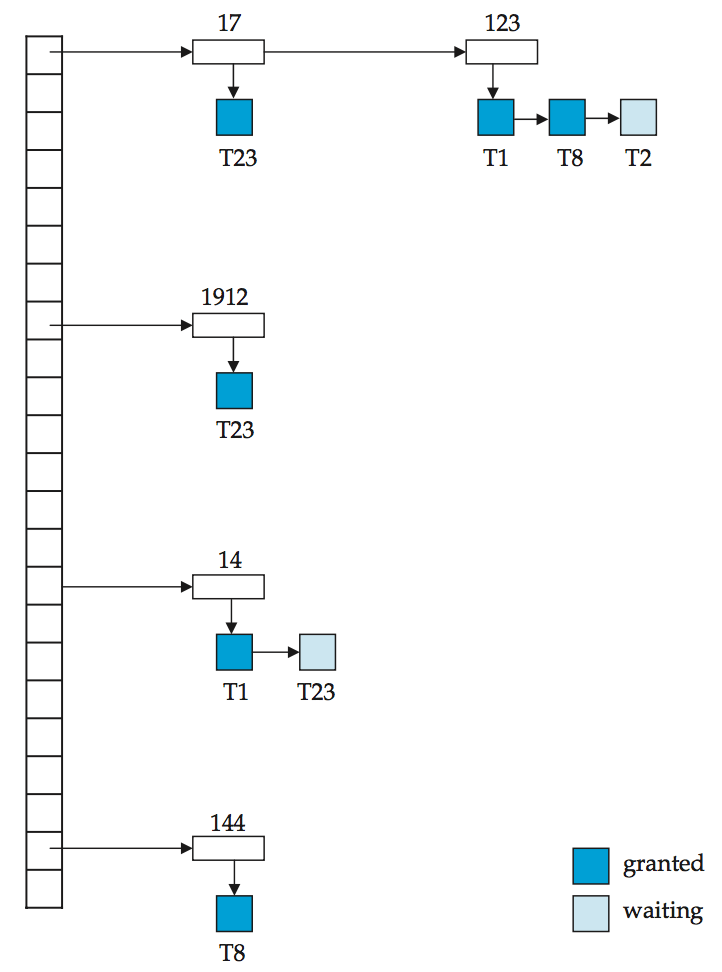
\includegraphics[width=0.4\textwidth]{images/lock-table}
\end{center}

The rules for constructing and manipulating such a lock table are pretty simple and comprehensible from the diagram. Each (lockable) data item is associated with a linked list. Entries in that linked list contain the transaction identifier and an flag to indicate granted or waiting.

If a request arrives for a data item for which there is no lock, then an entry is created and the request be immediately granted. If a lock already exists for that data item, a new entry is created. As for whether it is granted right away or not, compatibility must be checked. If it is compatible it may be granted; otherwise it must wait. 

When there is an unlock request, the entry for that transaction and data item are removed and, if possible, further requests are granted. If a transaction aborts, any locks (granted or not) are removed from the lock table.

This algorithm avoid the possibility of starvation, because the linked list imposes order on the request such that later requests always are enqueued after earlier ones~\cite{dsc}.

The graph based protocol in~\cite{dsc} is has to do with establishing a lock based protocol that uses a tree. To make this work, all data elements need to be assigned an identifier (an ID of some sort) which allows establishment of partial ordering on the data elements. The purpose is so that it is possible to enforce the rule that they are acquired in order.

You might recall this sort of protocol from the general discussion of deadlock in a concurrency context. In the examples, a simple deadlock is created when one thread locks \texttt{a} and then \texttt{b} and the other thread locks \texttt{b} and then \texttt{a}. The solution was to establish an ordering on the lockable elements (in that case, the alphabetical ordering seemed logical enough, but reverse alphabetical would work too). That works okay for names, but not everything has a name, and anything relatively simple like memory location of file location would work to impose an ordering.

The tree protocol is an example in~\cite{dsc} that works only for exclusive locks with four rules:

\begin{enumerate}
	\item The first lock by a transaction $T_{1}$ may be on any data item.
	\item Any other data item $d$ may be locked by $T_{i}$ only if the parent of $d$ is currently locked by $T_{i}$.
	\item Items may be unlocked at any time.
	\item A data item that has been locked and then unlocked by $T_{i}$ cannot later be locked again by $T_{i}$.
\end{enumerate}

The diagram below illustrates a potential ordering of data elements:

\begin{center}
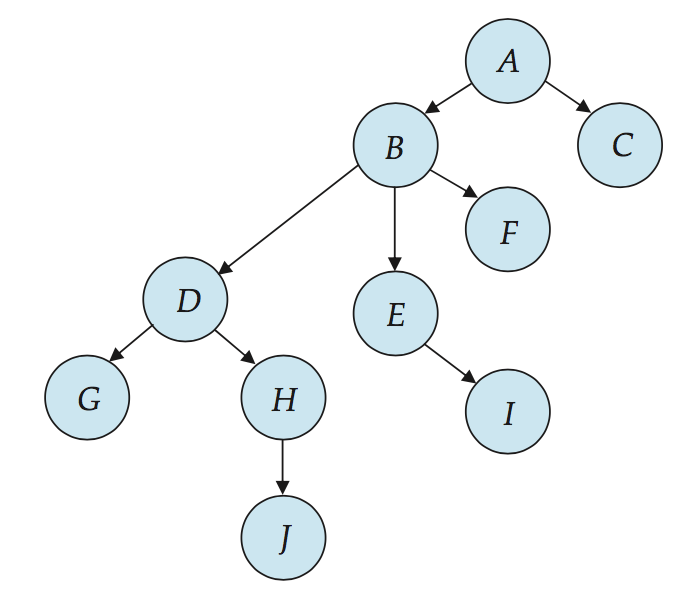
\includegraphics[width=0.5\textwidth]{images/tree-lock}\\
Tree structured ordering of data elements~\cite{dsc}
\end{center}

It is simple enough, when looking at this graph, to think of some schedules that are legal or illegal under this protocol. It can be shown that this protocol ensures freedom from deadlock. The reasoning is a fairly simple proof by contradiction: assume that a deadlock exists and then show a contradiction.

In~\cite{osc} is a proof that ordering the resources prevents deadlock in processes, and it is simple enough to modify for transactions. Let us say there is a function $f()$ that takes a data element and returns a unique identifier used for ordering. Assume a circular wait is present. Let the set of processes in the circular wait be $\{T_{0}, T_{1}, ... T_{n}\}$ and the set of resources (data elements locked) be $\{R_{0}, R_{1}, ... R_{n}\}$. The cycle is formed as: $T_{i}$ is waiting for resource $R_{i}$ and that resource is held by $T_{i+1}$. The exception is the case of $T_{n}$, which is waiting for resource $R_{n}$ that is held by $T_{0}$ (completing the cycle by wrapping around). Since Process $T_{i+1}$ holds resource $R_{i}$ while requesting $R_{i+1}$, this means $f(R_{i}) < f(R_{i+1})$ for all $i$. But this means that $f(R_{0}) < f(R_{1}) < ... < f(R_{n}) < f(R_{0})$. It cannot be the case that $f(R_{0}) < f(R_{0})$: a contradiction, meaning a circular wait cannot occur.

Use of the tree structured protocol does not, however, ensure recoverability or prevent cascades from occurring~\cite{dsc}. That means we need to also take steps, as earlier, to ensure that the schedule conforms to our other properties. The other negative here is that the database server might need to lock items other than the ones strictly necessary in the transaction.

Consider an example in the tree lock diagram above; if data elements $A$ and $J$ are needed, then items $B$, $D$, and $H$ also need to be locked to make this work. Moreover, it is very likely that we are going to lock the root of the tree, meaning that (most) transactions are effectively serialized. This is probably not a good thing.

The tree protocol is useful if the goal is to prevent deadlock from happening, but it is not e very good solution given the tradeoffs. It is more likely that we will just allow transactions to proceed and detect if they do get stuck, and if so, try to do something to fix it.

\bibliographystyle{alphaurl}
\bibliography{356}


\end{document}
